\documentclass[a4paper,14pt]{article}
\usepackage{graphicx} 
\usepackage{sectsty}
\usepackage{extsizes}


\linespread{1.5}

\begin{document}

\begin{titlepage}
	\centering
	{\bfseries\Large
		TAMANG OF NEPAL\\
		\vskip1cm


	}
	A Brief Ethniographic Report submitted to Paschimanchal Secondary School for fulfillment of Practical Requirement of Annual Board Examination of Grade XII (Humanities) taken by NEB Nepal
	%\vskip1cm


	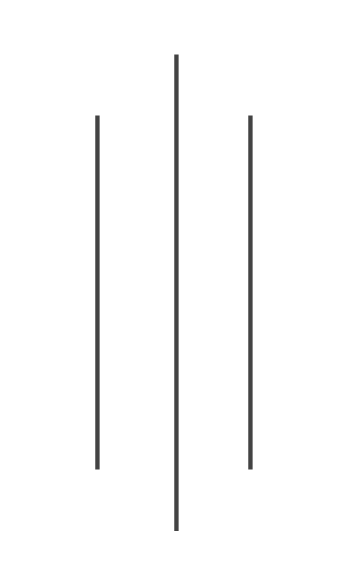
\includegraphics[width=3cm]{sample.png}
	%\vskip1cm

	\textbf{By:}

	Sunil Thapa\\
	Class Roll No. 46 \\
	Class: XII (Humanities)

	%\vskip0.5cm

	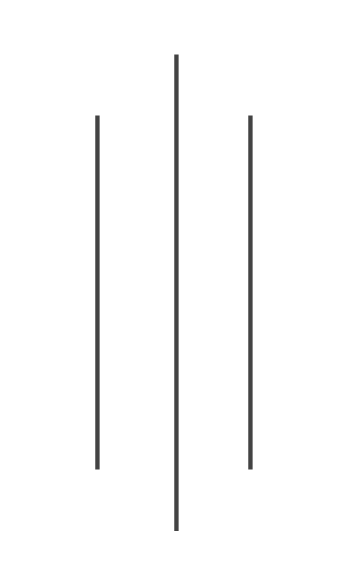
\includegraphics[width=3cm]{sample.png}

	%\vskip0.5cm

	Paschimanchal Secondary School \\
	Pokhara-4, Gairapatan \\
	2076
\end{titlepage}

\begin{flushleft}
	\section*{ACKNOWLEDGEMENT}
	I am highly indebted to my teacher Mr. Amrit Kumar Bhandari for his guidance and constant supervision as well as for providing necessary information regarding the project and also for his support on completing the project. I would like to express my gratitude towards my parents for their kind co-operation completion of this work.
	\vskip0.5cm


	I would like to express my special gratitude and thanks to those person of Tamang community for giving me such an attention and their precious time.
	\vskip0.5cm

	My thanks and appreciations also go to my classmate in developing the project and to the people who have project  and to the people who have willingly helped me out with their abilites.
	\vskip0.5cm

	Thank you





	\begin{flushright}
		Sunil Thapa
	\end{flushright}


	\newpage
	\tableofcontents

	\newpage

	\section{ORIGIN AND SETTLEMENTS}

	The Tamanga are a very ancient tribe of Nepal and are the original people of Yambu (Kathmandu Valley). Nepalese history states that the Enlightened Manjushree made an ancient abode of Tamang in Yambu. The ancient Tamang song - “Gyanaka Gyamse Phepkaziam" or "Appeared from China” says that the oldest tribe of Yambu is Tamang. There are dense Tamang settlements around Yambu even today.According to the version of the Dynasty of Nepal and Dr. Shetenkoko, Tamangs are the oldest tribe of Nepal. Dr. Anatoly Yakoblave Shetenko visited Nepal on an archaeological study programme under an agreement between Nepal and USSR. He discovered that the tools, weapons and artifacts that date back to the Stone Age (about 30,000 B.C.) at Budhanilkantha were the same as those found in Govy of Mongolia, Asia, and America. Presently such Mongolian artifacts dating back to the Stone Age are found in Yambu (Kathmandu, Budhanilkantha) which prove that the Mongolians (Tamangs) came by way of Tibet and the Himalayas to Nepal. It is evident that the Mongols were settled in Yambu (Kathmandu Valley) from the north more than 30,000 years ago. According to Janak Lal Sharma, "those Mongols that came from the north are today’s Tamangs." Earlier Tamangs were known by various terminologies. Among these, ‘Murmi’ is a popular term. Hamilton in 1802, Hudson in 1847, and Macdonald in 1989 have used the term ‘Murmi’ for Tamang people. Some scholars are of the opinion that during the regime of King Tribhuvan the then Prime Minister Bhim Shumsher had formally used the term ‘Tamang’ for the very first time under the request of Sardar Bahadur Jungabir, who was also from the Tamang nationality. In 13th century, King Boom Degon (1253-1280), who had ruled the present Mustang region of Nepal, has scriptured the word ‘Tamang’ in his genealogy. This is the oldest written document ever found about the usage of the word ‘Tamang’ that exclusively refers to the Tamang nationality of Nepal.There still prevails differences about the origin of the word ‘Tamang’. A common belief is that the word ‘Tamang’ has been derived from a Tibetan word "Tamag” which means ‘Ta’ referring to ‘horse’ and ‘Mag’ referring to ‘rider’. So Tamang are the ‘horse-riders or soldiers riding on horse. It is believed that after the Nepal-Tibet War some of the horse-riding soldiers of King Tsrong Tschong Gampo permanently settled in the Himalayan Hills of Nepal who were later recognized as the “Tamang” nationalities. But many scholars have opposed the above perspective that the Tamangs are the descendants of the horse-riding soldiers of King Tsrong Tschong Gampo. A foreign scholar Alexander MacDonald is one among them. According to him, Tamangs are the indigenous inhabitants of Nepal who were here before the state formation. He disagrees that Tamangs are the horse-riding soldiers of King Tsrong Tschong Gampo who were left behind after the Nepal-Tibet War. He puts forward his reasoning that there should be some mention of King Gampo in the genealogy of Tamang nationality if it was so. But nothing has been found yet.In their language, the Tibetans call Tamang people ‘Rongpo’ which means 'foreigners'. Obviously, it also justifies that Tamangs are the indigenous inhabitants of Nepal, not the horse-riding soldiers of King Tsrong Schong Gampo. A young scholar Ajitman Tamang redefines the Tibetan perspective of the word ‘Tamang’. He is of the view that in Tibetan ‘Ta’ means ‘entrance/gateway’ and ‘Mang’ means ‘large public or common people’. So, ‘Tamang’ in Tibetan means presence of large number of people at the entrance or boundary, which signifies the settlement of Tamang people in the border of Tibet i.e. in Nepal. It is also supported by the Tibetan usage of the word ‘Rongpo’ to Tamang, which means the foreigners, inhabited beyond the border of Tibet. Now it is obvious that the Tamangs are the indigenous inhabitants of Nepal, not the descendants of the horse-riding soldiers of King Tsrong Tschong Gampo as Tamang themselves do not possess the characteristics of a horse rider nor there a sign of their history directly associated with horses. Usage of the word ‘Tamang’ It is still in the root of the research from when the word ‘Tamang’ has been in use to refer to the Tamang nationality of Nepal.
	
	
	\newpage
	\section{POPULATION DISTRIBUTION}

	\begin{table}[htb]
		\centering
		\begin{tabular}{lllll}
			\cline{1-3}

			\multicolumn{1}{|l|}{\textbf{Ethnicity}} & \multicolumn{1}{l|}{\textbf{Population}} & \multicolumn{1}{l|}{\textbf{Total of Whole Population}} &  & \\ \cline{1-3}
			\multicolumn{1}{|l|}{Tamang}              & \multicolumn{1}{l|}{1,539,830}           & \multicolumn{1}{l|}{5.6\%}                                &  & \\ \cline{1-3}
		\end{tabular}
	\end{table}

	The given data is according to the Nepal's census, 2011 AD . However this is not a particularly accurate figure since the Tamangs who had written Lama or their family name on the census form were not counted as Tamang and many others have in the past changed their caste in order to escape the caste limitations placed upon them. The majority of the Tamang population lives in 8 Districts: Kavrepalanchowk, Makwanpur, Ramechhap, Dhading, Nuwakot, Rasuwa, Sindupalchowk, Dolakh. The language also predominates in 2 further Districts: Rasuwa and Makwanpur.


	\newpage
	\section{MAIN FEATURES OF SOCIO-CULTURAL LIFE}
	\subsection{LANGUAGE}


	Tamang langugage is a language used to collectively refer to a dialect cluster spoken mainly in Nepal, Sikkim, West Bengal (Mainly Darjeeling Districts, some parts of Assam and North East Region. It comprises Eastern Tamang, Northwestern Tamang, Southwestern Tamang, Eastern Gorkha Tamang, and Western Tamang. Lexical similarity between Eastern Tamang (which is regarded as the most prominent) and other Tamang languages varies between 81\% to 63\%. For comparison, lexical similarity between Spanish and Portuguese, is estimated at 89\%.Tamang likely split from the Tibetan languages some time before the 7th century.

	
	\newpage

	\subsection{RELIGION}
	Tamangs are Lama (Tibetan) Buddhists, as are most upper Himalayan peoples. Their religion is traditionally Bon Lamaism; a fusion of Shamanism and Buddhism. Bon is the pre Buddhist belief concentrated in Tibet and still widely practised although generally ignored in Western perceptions or descriptions of the area. They have gompas (monasteries) in every sizeable village. Every family has their special Buddhist god and book to worship every morning. The Tamangs retain jhankris (shamans) in addition to their lamas (priests). These jhankris perform certain rites such as trances and sacrifices to alleviate problems or assure good fortune.


	\newpage
	\subsection{FESTIVALS}
	Sonam Loshar is the main festival of the Tamangs and is celebrated in the month on Magh (February - March). It is celebrated to welcome the Tamang new year.

Colorful flags, printed Buddhist mantra cloths are put up in various places in villages and towns. The Tamangs have a genre of music called " Tamang Selo" that is performed with the Damplu instrument, also known as Damphoo Dance, having a brisk movement and rhythmic beat specific to the Tamangs.

The second most important festival is Saga Dawa (Buddha Jayanti) and is celebrated as a religious festival.

Dashain and Tihar (festival) is also celebrated with much enthusiasm by Tamangs.

\subsubsection{Lhosar - Celebrating The New Year }
The main festival celebrated by the Tamang community is Lhosar. Lhosar is a new year festival celebrated on the first day of the Lunar calendar (which usually happens in February). The community has 12 different animals as 12 years. On the first day of Lhosar people make figures of the 12 animals with flour. The exchange of traditional sweets made of buckwheat like Khapse and Aalum takes place among relatives and loved ones. The elders of the family also give their blessings in the form tika (rice mixed with yogurt).

	\newpage

	\subsection{RITUALS}

	\subsubsection{From Pregnancy Till Childbirth} :
In Tamang community, the rituals for the unborn child begins with the confirmation of the pregnancy. According to Buddhist tradition, before the birth of a child, religious rituals are performed for their protection against external vices. As long as the child is in the womb, it is believed that the parents of the unborn child should not sacrifice any animals. The Nwaran (naming ceremony) is performed within 3 days of childbirth by a Lama. The ritual can also be performed on the 11th day of the childbirth, if unfavourable circumstances arise. 

There is an utmost value of a Lama in every aspect of Tamang rituals. From birth to death, the presence and rituals performed by a Lama is considered supreme. Before the naming ceremony of the child, Dipchyang Pong (offering) is served to the Lama. The Lama then picks the ideal date for the ritual and performs purification or cleansing ritual for the child with Bonbo water. Bamboo is one of the major ritual practitioners in Tamang life. Bonbo have unique powers of sight and capture lost shadow-souls, revive life force and reveal the source of distress. The end of the ritual is marked with distribution of Bonbo water and fried rice flour among relatives. 
After birth, the next important ceremony in the Tamang community is the rice feeding ceremony. Daughters are fed rice at 5 months and sons are fed at 6 months. The eldest member of the family feeds the child with the beaks of the Mynah Bird. "It is believed that being fed with the beaks of the Mynah, the child develops a sweetness in the voice like a bird," said the Tamang scholar. 



\subsubsection{Young People}
Alongside the growth of the child, there are various norms and values to support the child socialize in the ad-hoc environment. Daughters are presented a "Syama," a pair of hand woven traditional clothes. In every odd year, the Lama presents the "Syama" to the daughters. After the Tamba, a societal leader in the Tamang community recites the origin of ”Syama" the daughter is given clothes. However, the tradition of "Syama" is fading away in recent times. Sons perform the Chewar, a head shaving ceremony. For sons, their part in family rituals and other practices come to value only after the Chewar. It should be done between 3rd day and 7 years of birth. An invitation for Chewar consisting of rice, beaten rice, wheat bread, alcohol and rooster is sent to the maternal uncle. The uncle then comes with new scissors, cap, white cloth belt, a cloth to cover the shaved head, plate, a pair of suits, offerings and a water pot as acceptance to the invitation and performs Chewar on his nephew. 

\subsubsection{Marriage} 
The marriage ceremony of the Tamang community is unique as well. In Tamang community, there is acceptance of marriage between maternal and paternal cousins. The Tamba represents the boy side of the family and takes bread, hen and alcohol as an offering to the girl's side of the family for marriage proposal. The acceptance of the offering denotes an affirmative answer while returning the offering denotes the opposite. 

The groom side brings an offering consisting of a 12 of any required elements to the bride's side of the family. There is a requirement of 12 Mohar paisa (1 mohar = 50 paisa and 100 paisa = Rs. 1), 12 dharni goat, (1 Dharni = 2.4 kg), 12 paathi rice (1 paathi = 4.5 kg) 12 paathi chyang (chyang is local alcohol) and 12 Bisa roti to perform marriage rituals. Another important ritual in the Tamang marriage is Chardam also known as Karjel Chol (giving away the virgin). The ritual consists of 1 mana (a pot of bronze to measure grains) rice, 1 paisa, drinks like jaad, raksi (local alcohol). A pair of pigeons is represented as family ancestors and the Chardam is performed. The pigeons are free to fly after the ritual is complete. If legend is to be believed, it is said that the marriage ceremony of the couple is not fully accepted until the Chardam is performed. 

The Tamang community prioritizes maternal power over paternal in case of marriage decisions. The bride's mother's decision is supreme. The community equally respects widow marriage. They encourage the widow to remarry the brother of her husband.  The decision to remarry remains in the hands of the widow. Mr. Rabindra Tamang, a Tamang scholar said that the community is also acceptable if the woman wishes to marry another man, while her husband is still alive. 

\subsubsection{Death}
Rituals performed for the deceased soul is also considered of great significance. These rituals are performed within 7 or 49 days of death. In the death of a married woman, her maternal family performs the closing ritual. "The woman is handed over to her mother's family after her death. The rituals are performed at the husband's house while the closing ritual 'Taashi' is to be done in the women's mother's house," says Rabindra Tamang. Tashi is the ritual process where the deceased is prayed to be sent to heaven. 




	\newpage

	\subsection{MUSIC}
	Tamang Selo  is a genre of Nepali folk song sung by the Tamang people and widely popular among the Nepali-speaking community in Nepal, in India, and around the world. It is usually accompanied by Tamang instruments, the Damphu, Madal and Tungna. A Selo could be very catchy and lively or slow and melodious and is usually sung to express love, sorrow and stories of day to day life.
	
	Hira Devi Waiba is hailed as the pioneer of Nepali folk songs and Tamang Selo. Her song "Chura ta Hoina Astura"  is said to be the first Tamang Selo ever recorded.Waiba has sung nearly 300 songs in a career spanning 40 years.




	\newpage
	\subsection{OVERALL ECONOMY AND ADAPTIVE STRATEGY}

	Tamang are made up of social groups associated with hereditary professions that provide ritual and economic services. Most people, living in compact traditional settlements, are self- sufficient as far as food is concerned. Tamangs living outside such settlements are generally very poor and they mainly work as porters, coolies for the trekkers and traders in the hill areas. They can not sustain on the cultivation on their marginal strip of land. Tamangs are very skillful in making woolen garments from sheep wool. Some of them are also trained to paint beautiful thankas while some of them are engaged in modern industry, business and service sectors.


	\newpage
	\subsection{ORNAMENTS}
	Dhungri, Fuli, Bulaki, Jantar and Red Muga are unique ornaments that highlight the beauty of women representing the Tamang community. 
	The female wears a kind of star shaped bracelet and bangles called mathi, chyap (finger ring), nhabi mhar (ear ornament), botil or alung (earring) and chaldang (lie sikree).

	\newpage
	\section{ROLE IN NATION BUILDING}
	Tamang People are belived to be the oldest handicrafts and woolen garment producer in Nepali civilization. They've started doing business in Nepal before  the mediaval period. In these days, Tamang people have maintained their legacy and continued to be the most creative handicraftsmen and garment producer in Nepal. Also, we can see that youth Tamang have shifted to foreign imployment contributing to nation remittance. 
	
	\newpage
	\section{RELATIONSHIP WITH OTHER CAST / ETHNIC GROUPS}
	Tamang People have decent relationship with other people. Generally, they don't allow marriage with caste of other people.
	

	\newpage
	\section{RECENT CHANGE IN THEIR EVERYDAY LIFE}
	Observing the Tamang People, we can analyze that Tamang are distributing their interests to several variations. Some are advancing their modern lifestyle leading to fade the interest towards traditions they used to follow. Migration is playing a key role for this. Abroad settlements plays a major factor which results the attraction towards foreign culture. People are advancing their interests to technology and modern finances. Due to such modern context, people are detaching their native cultural and traditional interests.



	\newpage

	\begin{thebibliography}{9}

		\bibitem{book}
		Dor Bahadur Bista
			[\textit{People of Nepal}].
		1987.

		
		\bibitem{sujanblog}
		Relationship Between Tamang and High Castes,
		\\\texttt{https://www.researchgate.net/publication/273817823_Changing_Relations_between_High_Castes_and_Tamang_in_Melamchi_Valley}

	\end{thebibliography}

\end{flushleft}
\end{document}